\graphicspath{{./content/breast/figures/}}

\subsection{Image formation, limitations and imaging perspectives}

\begin{frame}
\frametitle{Breast structures and appearance under US screening}
\vspace{-10pt}
\begin{columns}
  \begin{column}{.48\textwidth}
    \begin{figure}\centering
      \begin{adjustbox}
        {max size={\textwidth}{.60\textheight},keepaspectratio=true}
        \input{./content/breast/figures/breast.tikz}
      \end{adjustbox}
      \caption{Breast structure elements.}
    \end{figure}	
  \end{column}

  \begin{column}{.48\textwidth}
    \begin{overprint}
      \onslide<1|handout:0>
      \begin{figure}\centering
        \includegraphics[width=.75\textwidth]{tissue.pdf}
        \caption{ Scheme of the elements present in a Breast \ac{us} image.}
      \end{figure}	

      \onslide<2|handout:0>
      \begin{figure}\centering
        \includegraphics[width=.75\textwidth]{US.pdf}
        \caption{Ideal Breast \ac{us} screening.}
      \end{figure}	
    \end{overprint}
  \end{column}

\end{columns}
\end{frame}

\begin{frame}\frametitle{Breast structures and appearance under US screening}
%This slide needs to be parted into two slides or a dinamic one where first is olny analyzed specular reflection and seond the scattering.
\begin{columns}
\begin{column}{.48\textwidth}%\hspace{-1cm}
\begin{tikzpicture}[scale=1]%,every node/.style={draw,inner sep=0}]
\begin{scriptsize}
	 \node[anchor=south west,inner sep=0] at (0,0) {\includegraphics[trim = 300 350 800 1000, clip,height=7.5cm]{USscattering/master2.pdf}};
 
%    \draw[help lines,xstep=.5,ystep=.5] (0,0) grid (4,8);
%\foreach \x in {0,.5,1,...,4} { \node [anchor=north] at (\x,8) {\x}; }
%\foreach \y in {0,.5,1,...,8} { \node [anchor=east] at (0,\y) {\y}; });

\def\waveXCenter{2.1}
\def\waveIni{6.3}
\def\waveFin{1}
\def\waveAmplitud{.8}
  \draw[decorate, decoration={snake, segment length=15, amplitude=15},red] (2.03,6) -- (2.03,4.3);
  \draw[decorate, decoration={snake, segment length=15, amplitude=8},red] (2.03,4.3) -- (2.03,.9);
 
\draw 	(0.3,4.7) node[anchor=center] {$R=\frac{Z_2 - Z_1}{Z_2+Z_1}$}
			(0.3,4) node[anchor=center] {$T=\frac{2Z_2}{Z_2+Z_1}$}
			(3.2,4.7) node[anchor=west] {$Z_1$}
			(3.2,4) node[anchor=west] {$Z_2$};

\end{scriptsize}
\end{tikzpicture}
\end{column}

\begin{column}{.48\textwidth}
  \vspace{-10pt}
		\begin{figure}
\includegraphics[width=.7\textwidth]{US.pdf}
        \caption{Ideal Breast \ac{us} screening.}
		\end{figure}
\end{column}
\end{columns}
\end{frame}

\begin{frame}\frametitle{Breast structures and appearance under US screening}
%This slide needs to be parted into two slides or a dinamic one where first is olny analyzed specular reflection and seond the scattering.
\begin{columns}
\begin{column}{.48\textwidth}%\hspace{-1cm}
\begin{tikzpicture}[scale=1]
\begin{scriptsize}
\def\waveXCenter{2.1}
\def\waveIni{6.3}
\def\waveFin{1}
\def\waveAmplitud{.8}
  \draw[decorate, decoration={snake, segment length=15, amplitude=15},red] (2.03,6) -- (2.03,.9);
	 \node[anchor=south west,inner sep=0] at (0,0) {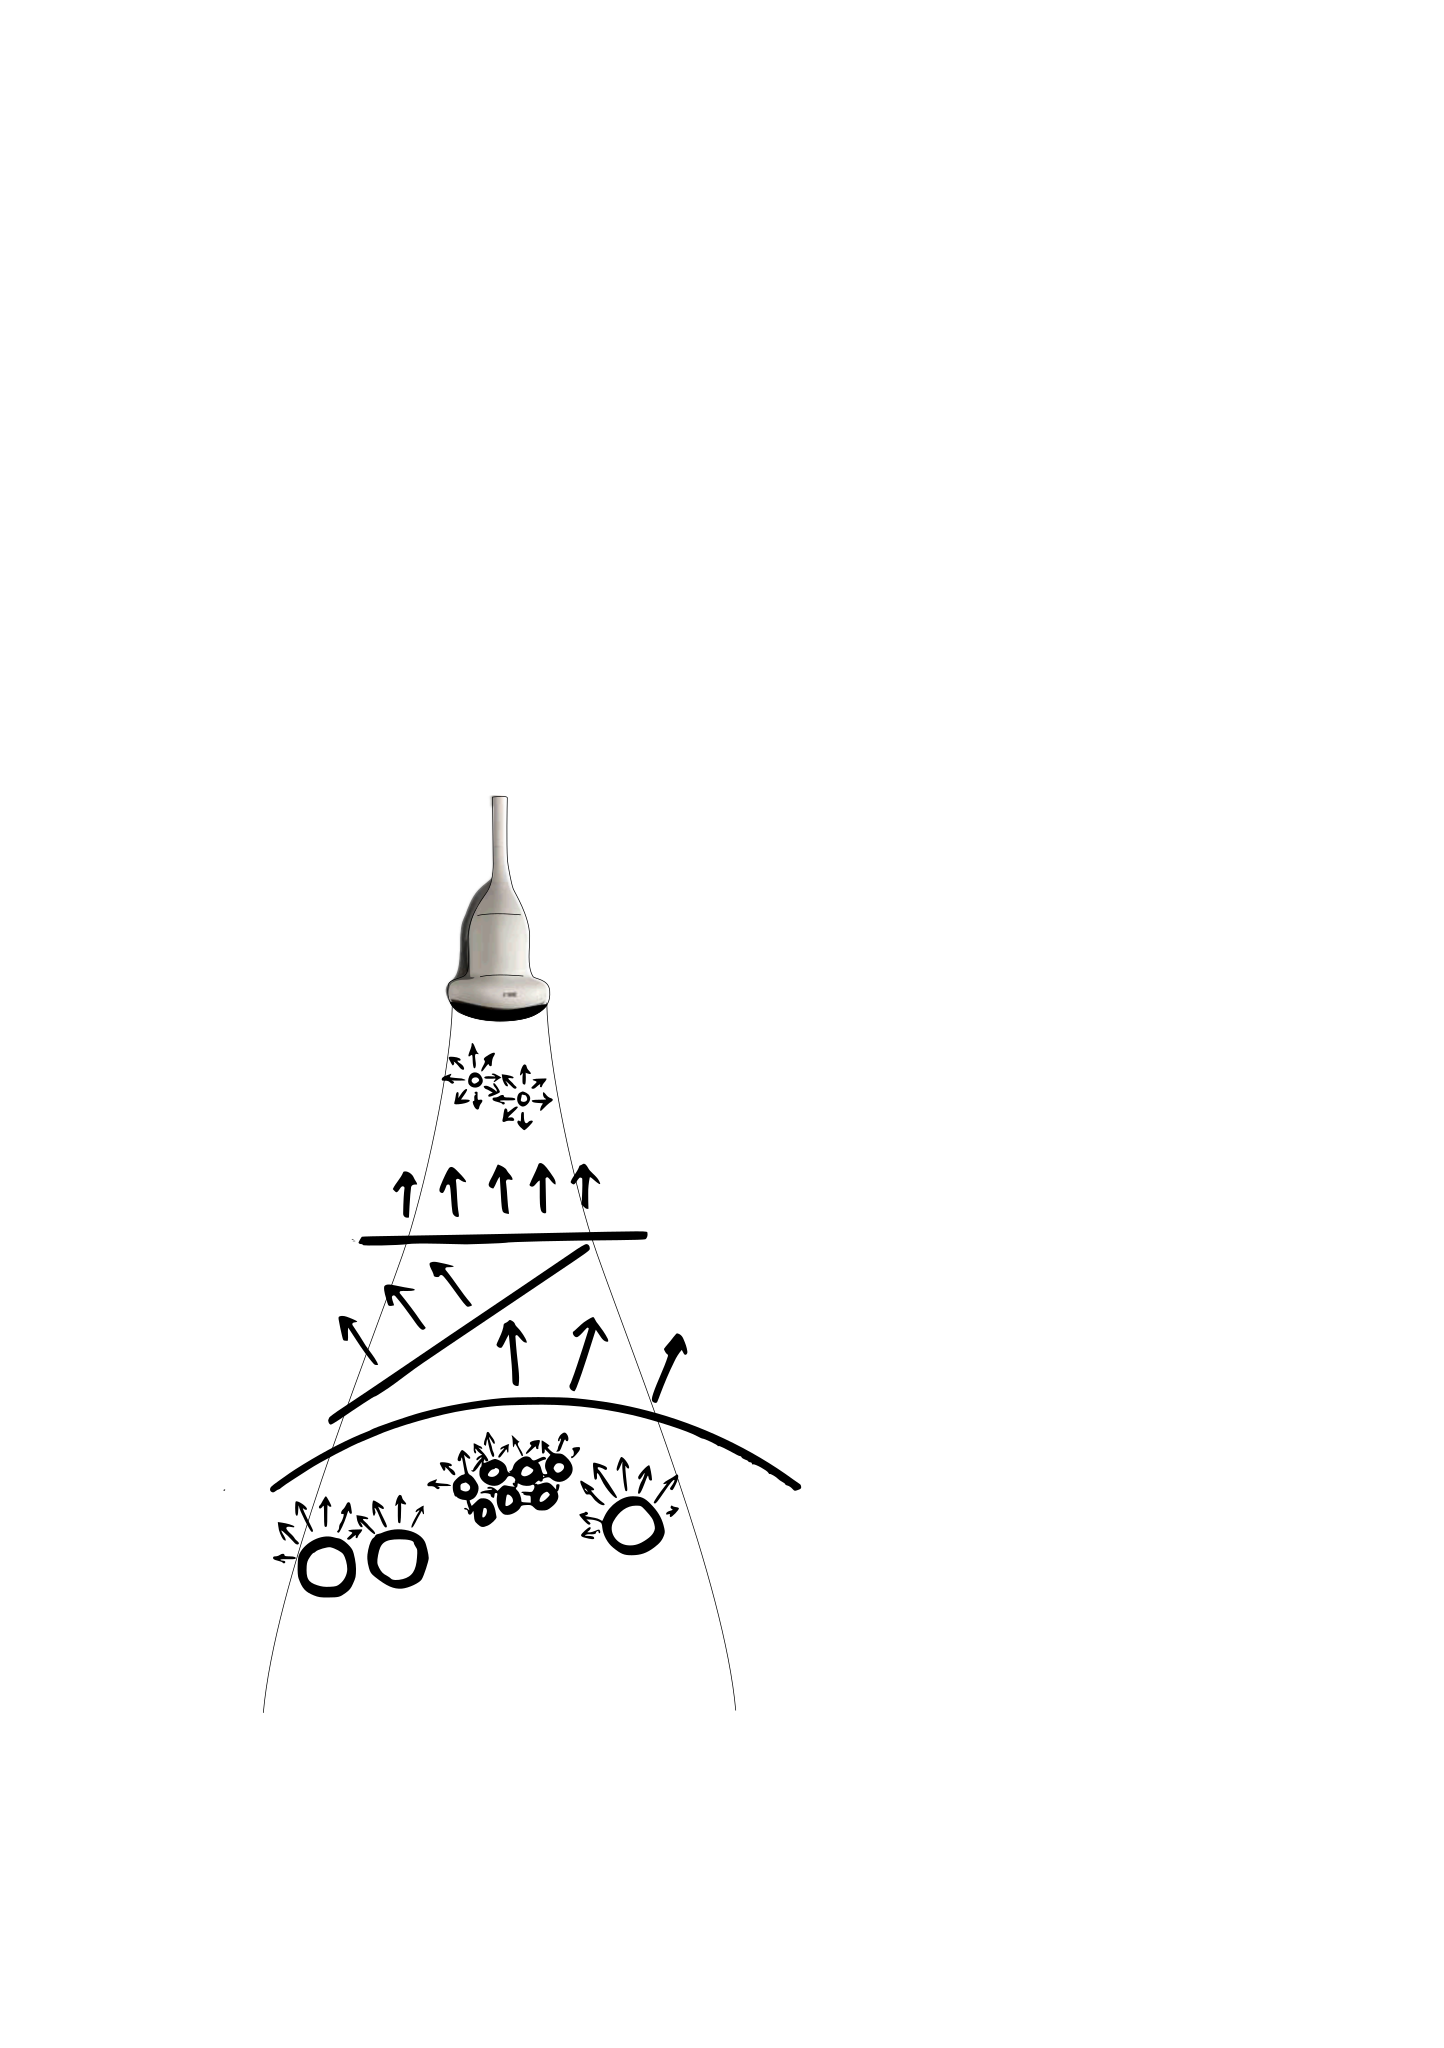
\includegraphics[trim = 300 350 800 1000, clip,height=7.5cm]{USscattering/master.pdf}};
 
%    \draw[help lines,xstep=.5,ystep=.5] (0,0) grid (4,8);
%\foreach \x in {0,.5,1,...,4} { \node [anchor=north] at (\x,8) {\x}; }
%\foreach \y in {0,.5,1,...,8} { \node [anchor=east] at (0,\y) {\y}; });


 
\draw 	(0.3,4.7) node[anchor=center] {$R=\frac{Z_2 - Z_1}{Z_2+Z_1}$}
			(0.3,4) node[anchor=center] {$T=\frac{2Z_2}{Z_2+Z_1}$}
			(3.2,4.7) node[anchor=west] {$Z_1$}
			(3.2,4) node[anchor=west] {$Z_2$};

\end{scriptsize}
\end{tikzpicture}
\end{column}

\begin{column}{.48\textwidth}
  \vspace{-10pt}
		\begin{figure}
\includegraphics[width=.7\textwidth]{US.pdf}
        \caption{Ideal Breast \ac{us} screening.}
		\end{figure}
\end{column}
\end{columns}
\end{frame}

\begin{frame}\frametitle{Breast structures and appearance under US screening}
  \centering
		\begin{figure}
		\includegraphics[height=.50\textheight]{sa1.png}~
		\includegraphics[height=.50\textheight]{sa2.png}
		\caption{ Ultrasound screening examples of two healthy breasts.}
		\end{figure}	
\end{frame}

\begin{frame}\frametitle{Elements degrading breast ultrasound images}
\begin{columns}
\begin{column}{.3\textwidth}
\begin{itemize}
\item Field of view
\item Weak edges
\end{itemize}
\end{column}
\begin{column}{.5\textwidth}
\begin{itemize}
\item ``Illumination'' inconsistency
\item Speckle
\end{itemize}
\end{column}
\end{columns}	

		\begin{figure}\centering
		\includegraphics[trim = 20 190 80 20, clip,height=.3\textwidth]{pit.jpg}\qquad
		\begin{tikzpicture}[scale=1]
		\draw[decorate, decoration={snake, segment length=15, amplitude=10},red] (1,1.6) -- (5.85,1.6);
			 \node[anchor=south west,inner sep=0] at (0,0) {\includegraphics[trim = 140 600 600 1150, clip,height=.3\textwidth]{USscattering/master90.pdf}};
		 \begin{tiny}
		  \draw 	(2.4,.5) node[anchor=north east] {$R=\frac{Z_2 - Z_1}{Z_2+Z_1}$}
					(2.4,.5) node[anchor=north west] {$T=\frac{2Z_2}{Z_2+Z_1}$}
					(2.3,2.5) node[anchor=south east] {$Z_1$}
					(2.4,2.5) node[anchor=south west] {$Z_2$};
		 \end{tiny}					
%		    \draw[help lines,xstep=.5,ystep=.5] (0,0) grid (4,4);
%		\foreach \x in {0,.5,1,...,4} { \node [anchor=north] at (\x,0) {\x}; }
%		\foreach \y in {0,.5,1,...,4} { \node [anchor=east] at (0,\y) {\y}; });
		
		\end{tikzpicture}
		\caption{ Elements related to the formation of the image. Left: Breast structures. Right: Image formation principles.}
		\end{figure}	
\end{frame}


\begin{frame}\frametitle{Elements degrading breast ultrasound images}
\setbeamercovered{transparent}
\begin{columns}
\begin{column}{.3\textwidth}
\begin{itemize}
\item<+> Field of view
\item<1-> Weak edges
\end{itemize}
\end{column}
\begin{column}{.5\textwidth}
\begin{itemize}
\item<+> ``Illumination'' inconsistency
\item<+> Speckle
\end{itemize}
\end{column}
\end{columns}	

\begin{overprint}
\onslide<1|handout:0>
		\vspace{15pt}
		\begin{figure} 
		\includegraphics[height=.28\textwidth]{sono/anon1704_9_1_CID}\hspace{1pt}
		\includegraphics[height=.28\textwidth]{sono/a110105_096_CDI}\hspace{1pt}
		\includegraphics[height=.28\textwidth]{sono/anon0101_0_3_H}
		\caption{Different fields of view. Left: Visualization of the main structures of the breast plus an intraductal carcinoma. Center: Ductal infiltrating carcinoma in a zoom view of the subcutaneous fat. Right: Large structured hematoma.}
		\end{figure}	

\onslide<2|handout:0>
		\vspace{15pt}
		\begin{figure} 
		\includegraphics[trim = 480 250 400 165, clip,height=.30\textheight]{sono/a20120525p062_1_1}\hspace{.5pt}
\includegraphics[trim = 92 75 88 85, clip,height=.30\textheight]{sono/00162}\hspace{.5pt}
\includegraphics[trim = 110 75 150 85, clip,height=.30\textheight]{sono/00166}
		\caption{Irregular sonification (illumination) in \ac{us} images. Left: Shadow produced by a solid mass. Center: Posterior enhancement. Right: Combined pattern. }
		\end{figure}	

\onslide<3|handout:0>
		\vspace{15pt}
		\begin{figure} 
		\includegraphics[trim = 0 0 25 0, clip,height=.31\textwidth]{speckle/005.png}\hspace{.5pt}
\includegraphics[trim = 480 350 400 165, clip,height=.31\textwidth]{speckle/physicPhantom.png}\hspace{.5pt}
\includegraphics[height=.31\textwidth]{speckle/cyst_sim.png}
		\caption{Speckle Noise produced by scatters. Left: Breast \ac{us} image. Center: Physical phantom of a cyst. Right: Synthetic phantom created with \emph{Field II}}
		\end{figure}	
%		\footnotetext[1]{\fullcite{jensen1996field}}
\end{overprint}
%\onslide<3> \footnotetext[1]{\fullcite{jensen1996field}}
\end{frame}


